% !TEX root = ../../Tesi_Triennale_PMNS.tex
\chapter[cWB]{cWB: proprietà dell'algoritmo per la rivelazione e la ricostruzione di segnali di onde gravitazionali}
\label{chapter:cwb}
\begin{center}
	$\smallsim 5/6$ pagine
\end{center}

Introduzione sull'algoritmo fatta nel paragrafo precedente, magari riprenderla velocemente.

Coherent analysis, significato e descrizione della likelihood: spiega quindi bene la differenza con gli algoritmi classici di confronto con segnali già modellati.

regolatori, antenna pattern

algoritmi utilizzati: wavelet transformation, (linear predicion error), mappa verosimiglianza, mappa energia coerente (con piccoli grafici esemplificativi)

(cenni sulla trasformazione di fase)

\begin{center}
	\begin{figure}[ht]
		\centering
		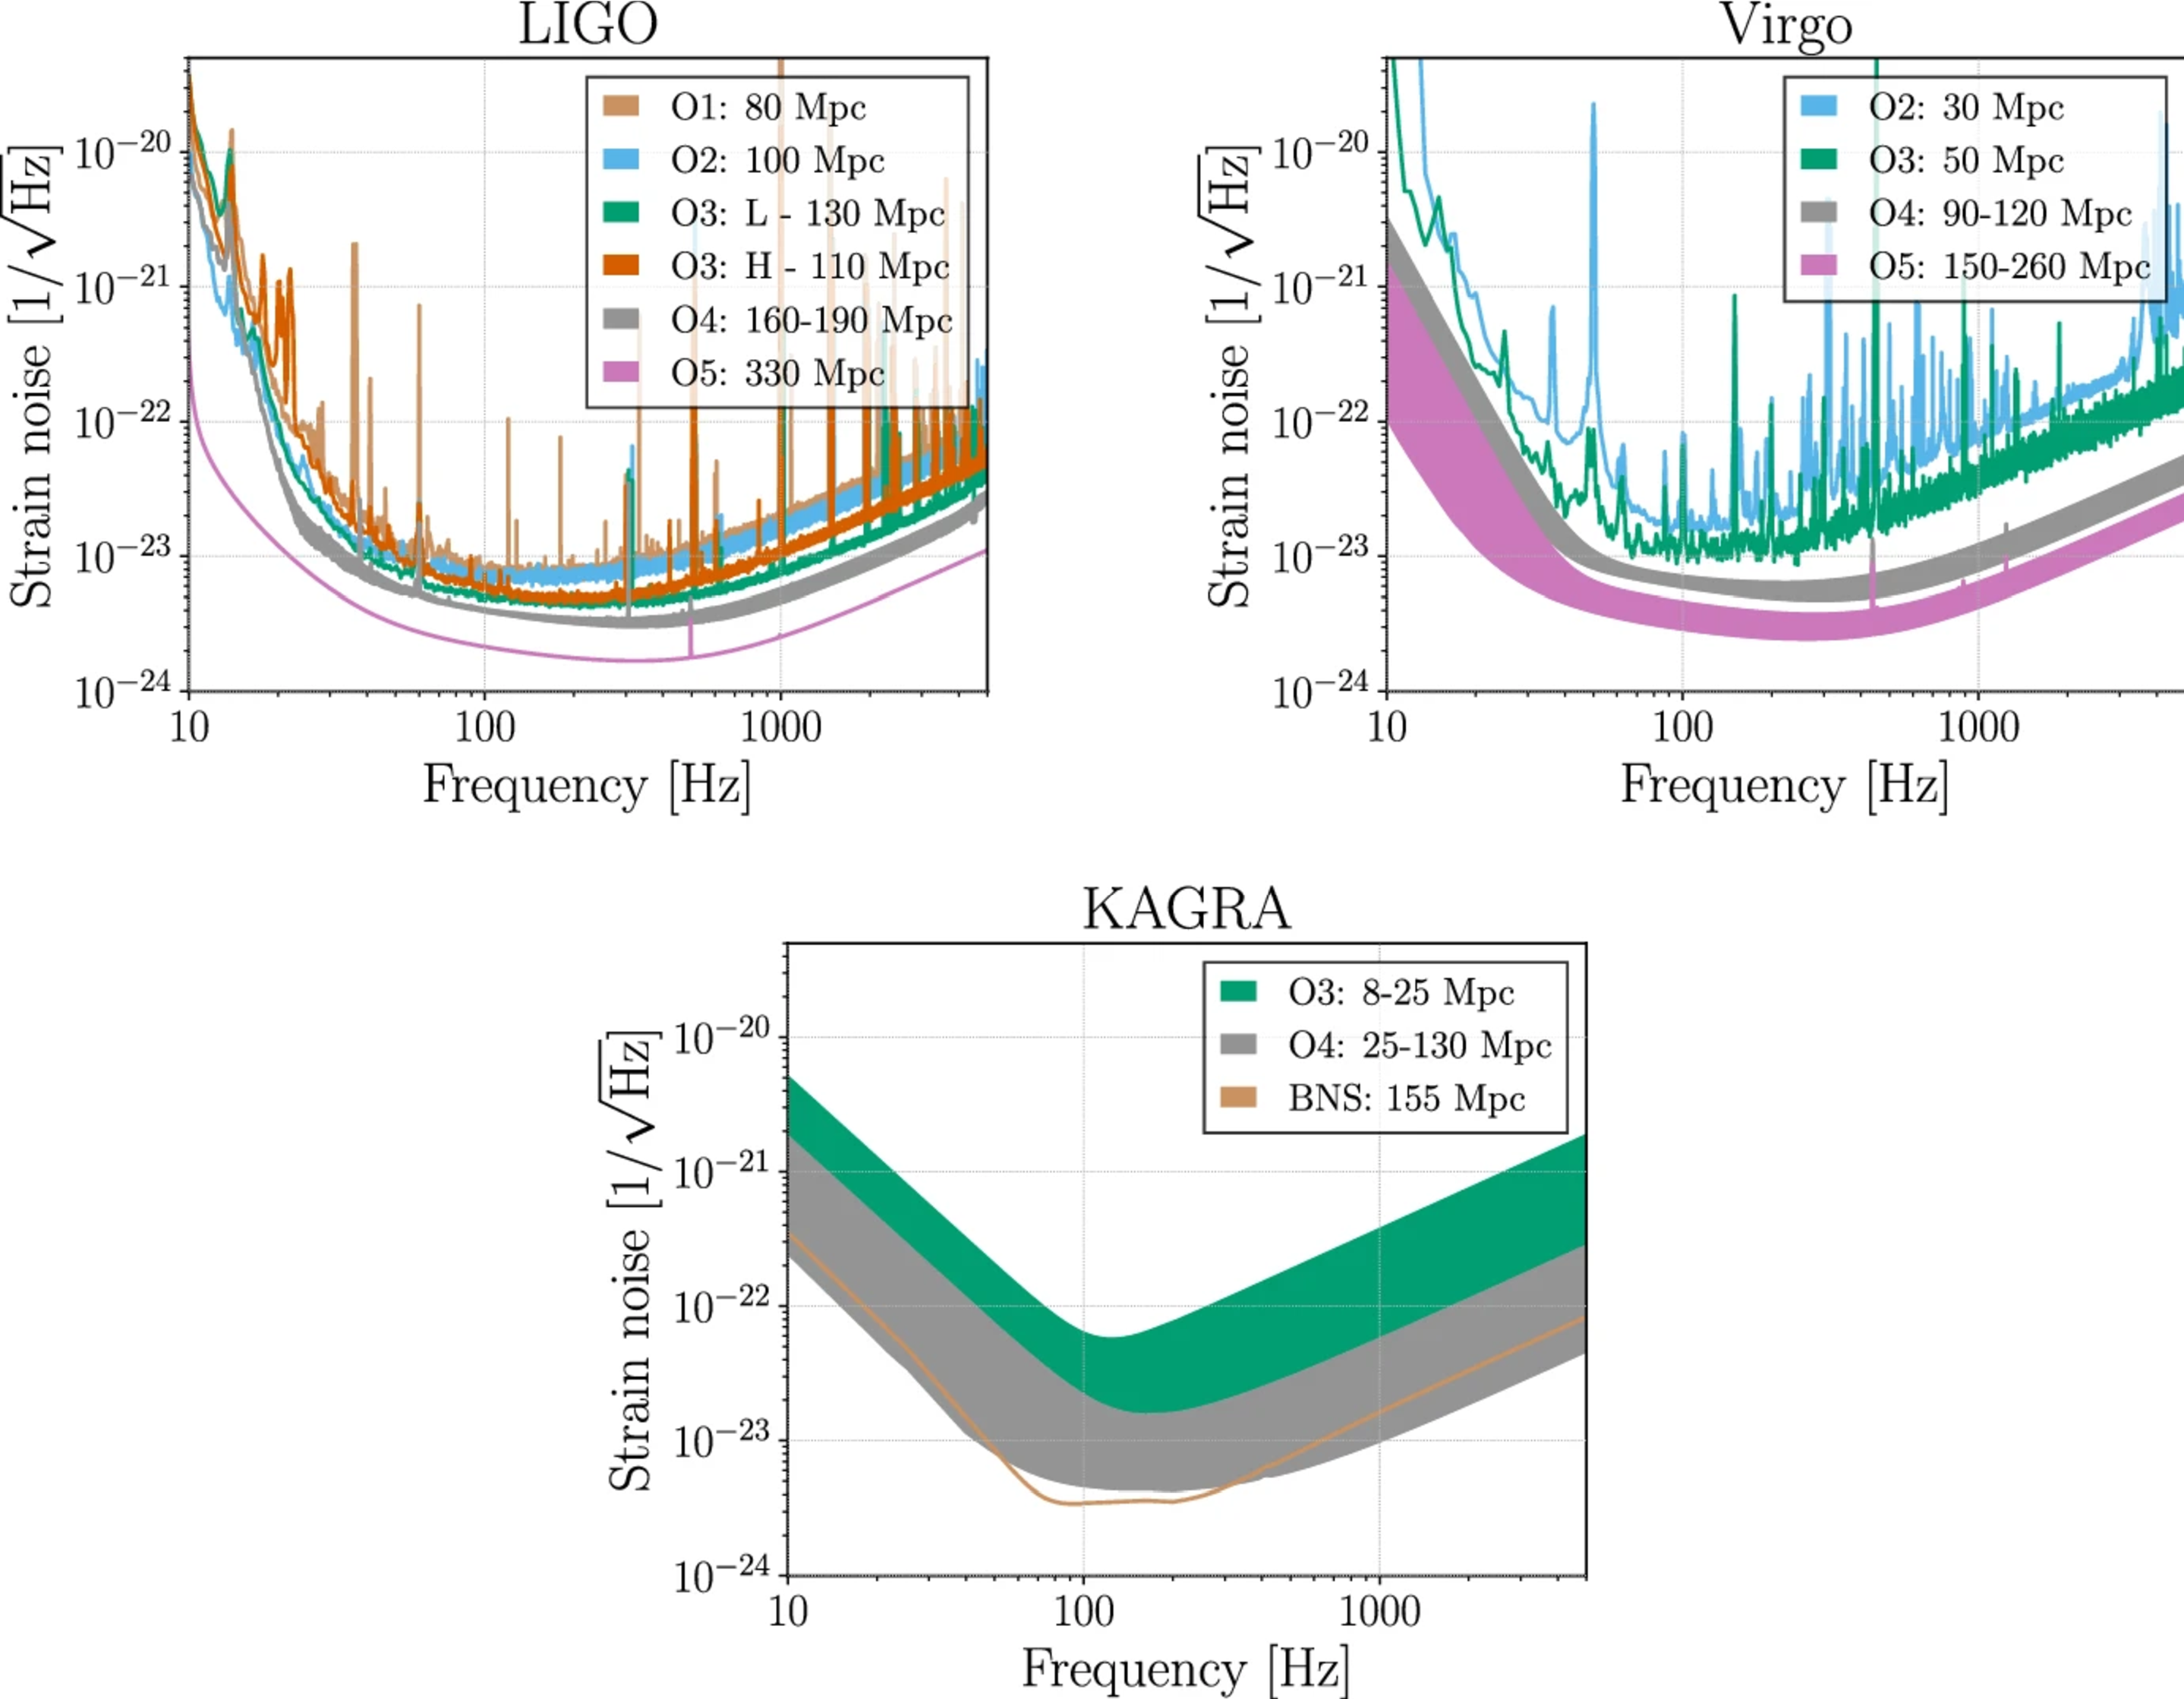
\includegraphics[scale=0.25, angle=0]{figures/Capitolo_3/noiseO4.pdf}
		\setlength{\belowcaptionskip}{-20pt}
		\caption{Prospetti \cite{Abbott_2020}}
		\label{fig:noiseO4}
	\end{figure}
\end{center}

\lipsum[3]\cite{Abbott_2017a}.

\lipsum[4]\cite{Klimenko_2008}.

\lipsum[6]\cite{Klimenko_2016}.